\documentclass[10pt,parskip=half]{scrartcl}

\usepackage{url}

% package for code formatting 
\usepackage{listings}
\usepackage{xcolor}

% This is an example for how code formatting could be customised 
\definecolor{codegreen}{rgb}{0,0.6,0}
\definecolor{codegray}{rgb}{0.5,0.5,0.5}
\definecolor{codepurple}{rgb}{0.58,0,0.82}
\definecolor{backcolour}{rgb}{0.95,0.95,0.92}

\lstdefinestyle{mystyle}{
	backgroundcolor=\color{backcolour},   
	commentstyle=\color{codegreen},
	keywordstyle=\color{magenta},
	numberstyle=\tiny\color{codegray},
	stringstyle=\color{codepurple},
	basicstyle=\ttfamily\footnotesize,
	breakatwhitespace=false,         
	breaklines=true,                 
	captionpos=b,                    
	keepspaces=true,                 
	numbers=left,                    
	numbersep=5pt,                  
	showspaces=false,                
	showstringspaces=false,
	showtabs=false,                  
	tabsize=1
}

\lstset{style=mystyle}

% I use this package to insert example images 
\usepackage{graphicx}

% I use this package to generate dummy text
\usepackage{lipsum}

% package for subfigures 
\usepackage{subcaption} 

% For clickable references/links, if you don't like the colourful box around your link, use \usepackage[hidelinks]{hyperref} 
\usepackage{hyperref} 

% booktabs package for pretty tables
\usepackage{booktabs}

% package for multirow tables
\usepackage{multirow}

% include this to use Tikz
\usepackage{tikz}

% define some custom shortcuts for my Tikz figure
\newcommand{\hk}{\ensuremath{\mathit{HK}}}
\newcommand{\tk}{\ensuremath{\mathit{TK}}}
\newcommand{\vk}{\ensuremath{\mathit{VK}}}
\newcommand{\sk}{\ensuremath{\mathit{SK}}}

% package for mathematical formulas and matrices
\usepackage{amsmath} 

% this package and the line underneath resets counter for my equations for every new equation environment
\usepackage{etoolbox}
\AtBeginEnvironment{align}{\setcounter{equation}{0}}

% for perfectionists, this makes your text look nicer
\usepackage[activate={true,nocompatibility},final,tracking=true,kerning=true,spacing=true,factor=1100,stretch=10,shrink=10]{microtype}


% spellchecker
\usepackage[english]{babel}

\begin{document}
	
% this command gives me a table of contents 
\tableofcontents
% with this command, table of content is displayed on it's own page
\pagebreak

\section{Code Formatting}

	\begin{figure}[htp]
		\begin{lstlisting}[language=java]
		class HelloWorld {
			public static void main(String[] args) {
				System.out.println("Hello World!"); 
				// Hello World!
			}
	}
	\end{lstlisting}
\caption{Hello world java program}
\end{figure}



\begin{figure}[htp]
	\lstinputlisting[language=java]{hello_world.java}
	\caption{Hello world java program loaded from file}
\end{figure}

\section{Tables}
\begin{table}[h]
	\centering %with this I can center my figure 
\begin{tabular}{ccc} \toprule 
	A & B & C \\
	\midrule 
	a&b&c \\ \cmidrule{1-1} % \cmidrule gives us a rule from column 1-1, I could also set it from 1-3 if I want a rule under a, b and c 
	1&2&3\\ \bottomrule
\end{tabular}
\caption{Small table}
\end{table}

\begin{table}[h]
	\centering
	\begin{tabular}{lllll}
		\toprule
		\multirow{2}{*}{Models} & \multicolumn{3}{c}{Metric 1} & Metric 2\\
		\cmidrule{2-4} \cmidrule{5-5} \\
		{} & precision & recall & F-score  & R@10 \\
		\midrule
		model 1 & 0.67  & 0.8 & 0.729  & 0.75 \\
		model 2 & 0.8 & 0.9 & 0.847 & 0.85 \\
		\bottomrule
	\end{tabular}
\caption{Multiline table taken from \href{https://jdhao.github.io/2019/08/27/latex_table_with_booktabs/}{this tutorial}}
\end{table}




\section{Figures and Subfigures}

When placing figures or tables (also known as floats), there are a few different options you can specify: \\
\begin{itemize}
	\item \textbf{h} means \emph{here} $\rightarrow$ your float should be placed where you wrote it if there is enough space
	\item \textbf{t} means that the float is allowed to go into the \emph{top} area
	\item \textbf{b} means that the float can go in the \emph{bottom} area
	\item \textbf{p} means that the float should be placed on a page which only contains other floats. 
\end{itemize}

For more information, you can also read \href{https://tex.stackexchange.com/questions/39017/how-to-influence-the-position-of-float-environments-like-figure-and-table-in-lat/39020#39020}{this detailed stack exchange reply}. 

I can refer to a whole figure, e.g. Figure~\ref{fig:whole_fig} or a subfigure, e.g. Figure~\ref{fig:figure_1}. 

\begin{figure}[htp]
	\begin{subfigure}{0.3\textwidth}
		\includegraphics[width=0.9\linewidth]{example-image-a}
		\caption{Figure 1}
		\label{fig:figure_1}
	\end{subfigure}
\begin{subfigure}{0.3\textwidth}
	\includegraphics[width=0.9\linewidth]{example-image-b}
	\caption{Figure 2}
\end{subfigure}
\begin{subfigure}{0.3\textwidth}
		\includegraphics[width=0.9\linewidth]{example-image-c}
	\caption{Figure 3}
\end{subfigure}
\caption{3 Figures next to each other}
\label{fig:whole_fig}
\end{figure}

\section{TikZ}

	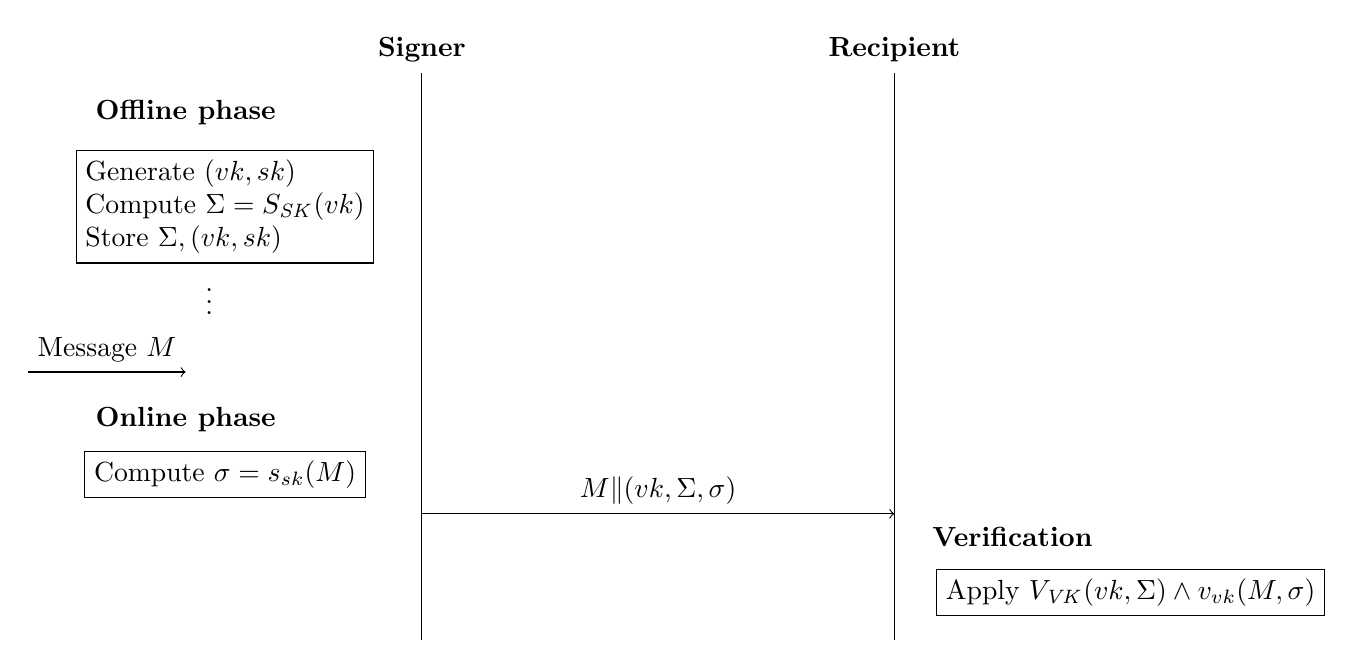
\begin{tikzpicture}
	\draw (-3,0) -- (-3,-7.2) (3,0) -- (3,-7.2);
	\node at (-6,-0.5) {\textbf{Offline phase}};
	\node[draw, align=left]  at (-5.5, -1.7) {Generate $(vk, sk)$ \\ Compute $\Sigma = S_{\sk}(vk)$ \\ Store $\Sigma, (vk, sk)$};
	\node at (-5.7,-2.8) {$\vdots$};
	\node at (-3,.3) {\textbf{Signer}};
	\node at (3,.3) {\textbf{Recipient}};
	\draw[->] (-8,-3.8) -- node[midway,above] {Message $M$} (-6,-3.8);
	\draw[->] (-3,-5.6) -- node[midway,above] {$M \Vert (vk, \Sigma, \sigma)$} (3,-5.6);
	\node at (-6,-4.4) {\textbf{Online phase}};
	\node[draw, align=left]  at (-5.5, -5.1) {Compute $\sigma = s_{sk}(M)$};
	\node at (4.5,-5.9) {\textbf{Verification}};
	\node[draw, align=left]  at (6, -6.6) {Apply $V_{\vk}(vk, \Sigma) \wedge  v_{vk}(M,\sigma)$};
\end{tikzpicture}

Example of a sequence diagram drawn with TikZ. \\

There are many example images for TikZ online. I gave you a few sources under useful links. When you want to draw something with TikZ, it makes sense to look for similar examples and to just modify them. This is what I did for this sequence diagram.

\section{Formulas and Matrices}

One example for a matrix: \\

\[\Phi = \begin{bmatrix} 
	\phi_0(x_1) & \dots  & \phi_{M-1}(x_1)\\
	\vdots & \ddots & \vdots\\
	\phi_0(x_N) & \dots  & \phi_{M-1}(x_N) 
\end{bmatrix}
= \begin{bmatrix} 
	\phi(x_1)^T \\
	\vdots \\
	\phi(x_N)^T
\end{bmatrix}
\] \\


In LaTeX, there are different ways to display mathematical expressions. Inline equations/mathematical terms appear directly in our text, e.g. $y = {y_1,\ldots ,y_N}$. \\ 

We can also use display mode which shows the formula in it's own line. Here we have two formulas set in display mode: \\ 

% we can use \[ \] around our formula 
The first one is unnumbered: 
\[E[\mu_{ML}] = E[\frac{1}{N}\sum_{n=1}^{N}x_n] = \mu\]
% as an alternative, we can also use the equation environment
% \begin{equation*}...\end{*equation} gives us an unumbered equation, if we leave out the *, we can get numbered equations 
We can also add numbering to our formulas: 
\begin{equation}[\sigma^2_{ML}] = E[\frac{1}{2}\sum_{n=1}^{N}(x_n - \mu_{ML})^2] = \frac{N-1}{N} \sigma^2\end{equation}


By using the \emph{aligned} command, we can align multiple formulas underneath each other. We can also use labels to refer to a specific line, e.g. see Equation~\ref{eq:line1}. 

\begin{align}
	E &= \frac{1}{2} \sum_{n=1}^{N}(t_n - \phi(x_n)^T \textbf{w})^2 \label{eq:line1} \\
	&= \frac{1}{2}(\mathbf{t} - \mathbf{\Phi w})^T(\mathbf{t} - \mathbf{\Phi w}) \\
	&= \frac{1}{2} (\mathbf{t}^T\mathbf{t} - 2\mathbf{w}^T\mathbf{\Phi}^T\mathbf{t} + \mathbf{w}^T\mathbf{\Phi}^T\mathbf{\Phi w}) \\
	0 = \nabla_wE &= \mathbf{\Phi}^T\mathbf{\Phi w} - \mathbf{\Phi}^T \mathbf{t} \\
	w &= (\mathbf{\Phi}^T\mathbf{\Phi})^{-1}\mathbf{\Phi}^T \mathbf{t}
\end{align}


\section{Example text with microtype}

The microtype setting makes the edges of your text look nice and smooth, see example text below. \\

\textbf{Example text:}

\lipsum[2-4]






\section{Useful Links} 
\begin{itemize}
\item \href{https://de.overleaf.com/learn/latex/How_to_Write_a_Thesis_in_LaTeX_(Part_3)%3A_Figures%2C_Subfigures_and_Tables#Subfigures}{Overleaf Tutorial for tables and figures}
\item \href{https://golatex.de/wiki/booktabs}{Some more information on tables with booktabs}
\item \href{https://jdhao.github.io/2019/08/27/latex_table_with_booktabs/}{Another tutorial for tables}
\item \href{https://texample.net/tikz/examples/}{Good source of TikZ examples}
\item \href{https://tikz.net/}{More TikZ examples}
\item \href{https://www.overleaf.com/learn/latex/TikZ_package}{Tutorial for basic TikZ features}
\item \href{https://www.resurchify.com/latex_tutorial/latex_alignment.php}{Tutorial for formulas}
\item \href{https://en.wikibooks.org/wiki/LaTeX/Advanced_Mathematics}{Guide on formatting mathematical formulas}
\item \href{http://www.khirevich.com/latex/microtype/}{More information on what microtype does for you}
\end{itemize}




	
\end{document}